% \subsection{Résolution d'équation différentielle : dynamique du bouchon flottant}

Ce sujet concerne la dynamique d'un bouchon en liège flottant dans un verre d'eau (voir figure suivante).% On considère un bouchon en liège cylindrique de révolution flottant dans un verre d'eau. 

\bigskip{}

\begin{minipage}{0.45\textwidth}
% \begin{figure}
\begin{center}
    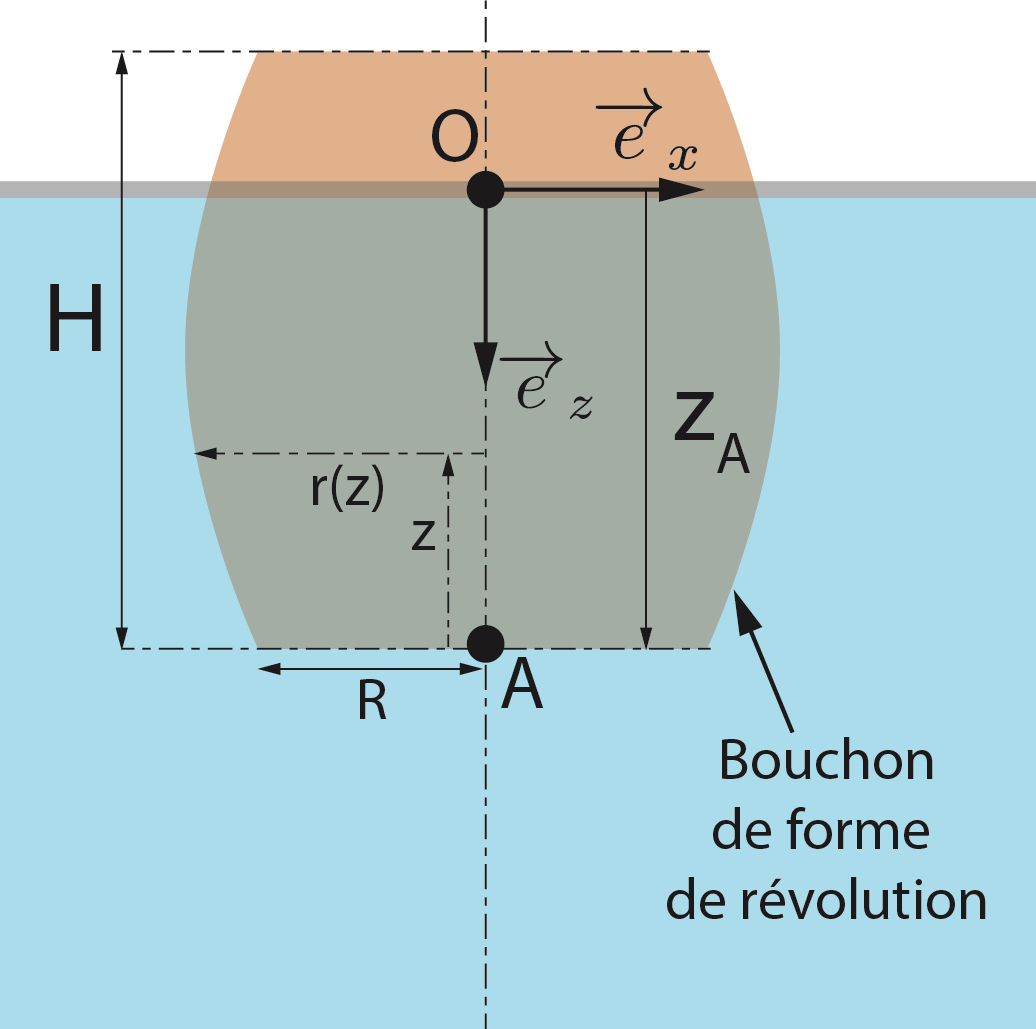
\includegraphics[width=1.0\textwidth]{parametrage.jpg}
% \caption{Paramétrage du problème}
% \label{EQD-003:fig:parametrage}
\end{center}
% \end{figure}
\end{minipage}
\begin{minipage}{0.45\textwidth}
On note : 
\begin{itemize}
\item $R$ le rayon de la base du bouchon ;
\item $\rho_e$ la masse volumique de l'eau ;
\item $\rho_b$ la masse volumique du bouchon ;
\item $z_A(t)$ la position verticale du bas du bouchon selon la direction $\overrightarrow{e}_z$ qui dépend du temps $t$ par rapport à $O$ (point situé sur la surface de l'eau);
\item $H$ la hauteur du bouchon.
\end{itemize}
\end{minipage}

\bigskip{}

Le bouchon possède une symétrie de révolution. Ainsi, son rayon, noté $r(z)$, dépend de la coordonnée $z$ de la manière suivante : 
\begin{equation*}
    r:\fct{[0,H]}{\R,}{z}{R\cdot \left[1+0,1\cdot \sin\left(\pi\cdot\dfrac{z}{H}\right)\right].}
\end{equation*}


Le volume immergé du bouchon dépend de la position $z_A$ et est donné par la relation suivante: 

\begin{equation*}
V_i(z_A)=
\left\{
\begin{array}{rcl}
0&\text{si}& z_A < 0~;\\
\\
\pi\cdot \displaystyle\int_{z=0}^{z_A}\left(r(z)\right)^2\mathrm{d}z&\text{si}& 0\leq z_A \leq H~;\\
\\
\pi\cdot \displaystyle\int_{z=0}^{H}\left(r(z)\right)^2\mathrm{d}z&\text{si}& z_A > H.
\end{array}
\right.
\end{equation*}

On note $V$ le volume total du bouchon correspondant à $V_i(H)$.

Le théorème de la résultante dynamique appliqué au bouchon selon la direction $\overrightarrow{e}_z$ donne : 

\begin{equation}\tag{$\mathscr{E}$}\label{EQD-003:eq:eqn_diff}
M\cdot \dfrac{\mathrm{d}^2z_A}{\mathrm{d}t^2}(t)=P-F_p\left(z_A(t)\right)+F_v\left(z_A(t),\dfrac{\mathrm{d}z_A}{\mathrm{d}t}(t)\right).
\end{equation}



Les grandeurs suivantes interviennent dans l'équation~\eqref{EQD-003:eq:eqn_diff}.
\begin{itemize}
\item[$\bullet$] $M=\rho_b\cdot V$, la masse du bouchon (égale au produit de sa masse volumique avec son volume).
%%\item Pour un cylindre de révolution, on rappelle : $V=\pi \cdot R^2\cdot H$
\item[$\bullet$] $P=\rho_b\cdot V\cdot g$, le poids du bouchon.
\item[$\bullet$] $g$, l'accélération de la pesanteur.
\item[$\bullet$] $F_p$, la force de poussée. Elle est égale au produit de la masse volumique de l'eau ($\rho_e$) avec $g$ et du volume immergé ($V_i(z_A(t))$), \emph{i.e.}  
\begin{equation*}
F_p(z_A(t))=\rho_e\cdot g\cdot V_i(z_A(t)).
\end{equation*}
\item[$\bullet$] $F_v\left(z_A(t),\dfrac{\mathrm{d}z_A}{\mathrm{d}t}(t)\right)$ est la force de frottement visqueux. Elle est donnée par la formule 
\begin{equation*}
    F_v\left(z_A(t),\dfrac{\mathrm{d}z_A}{\mathrm{d}t}(t)\right)=-\dfrac{1}{2}\rho_e\cdot C_x\cdot S\left(z_A(t),\dfrac{\mathrm{d}z_A}{\mathrm{d}t}(t)\right)\cdot \left(\dfrac{\mathrm{d}z_A}{\mathrm{d}t}(t)\right)^2.
\end{equation*}

% \begin{align*}
% 
% \left\{
% \begin{array}{l}
% 0\;\text{si }z_A(t)\leq0\\
% \\
% \;\text{si } \dfrac{\mathrm{d}z_A}{\mathrm{d}t}(t)\geq 0\;\text{et }z_A(t)>0\\
% \\
% +\dfrac{1}{2}S\cdot C_x\cdot S\left(z_A(t),\dfrac{\mathrm{d}z_A}{\mathrm{d}t}(t)\right)\cdot \left(\dfrac{\mathrm{d}z_A}{\mathrm{d}t}(t)\right)^2\;\text{si } \dfrac{\mathrm{d}z_A}{\mathrm{d}t}(t)\leq 0\;\text{et }z_A(t)>0\\
% \end{array}
% \right.
% \end{align*}
\item[$\bullet$] $S\left(z_A(t),\dfrac{\mathrm{d}z_A}{\mathrm{d}t}(t)\right)$ est la surface apparente du bouchon vis-à-vis du fluide et est définie de la manière suivante. 

\begin{itemize}
\item[$\ast$] Si le bouchon est totalement hors de l'eau, cette surface est nulle. 
\item[$\ast$] Si le bouchon descend et est (au moins partiellement) immergé  :
\begin{itemize}
\item si $0\leq z<H/2$, $S\left(z_A(t),\dfrac{\mathrm{d}z_A}{\mathrm{d}t}(t)\right) = \pi\cdot r(z)^2$,
\item si $z \geq H/2$,  $S\left(z_A(t),\dfrac{\mathrm{d}z_A}{\mathrm{d}t}(t)\right) = \pi\cdot r(H/2)^2$.
\end{itemize}
\item[$\ast$] Si le bouchon remonte et est (au moins partiellement) immergé  :
\begin{itemize}
\item si $0\leq z<H/2$, $S\left(z_A(t),\dfrac{\mathrm{d}z_A}{\mathrm{d}t}(t)\right) = 0$.
\item si $H/2\leq z \leq H$, la surface à prendre en compte est celle de la couronne  : $S\left(z_A(t),\dfrac{\mathrm{d}z_A}{\mathrm{d}t}(t)\right) = - \pi\cdot \left(r(H/2)^2-r(z)^2\right)$
\item si $z > H$, $S\left(z_A(t),\dfrac{\mathrm{d}z_A}{\mathrm{d}t}(t)\right) = - \pi\cdot r(H/2)^2$. 
\end{itemize}
La force de frottement s'opposant au mouvement, si le bouchon remonte, la résultante de cette force selon la direction $\overrightarrow{e}_z$ est positive, d'où le signe $-$ placé ici. 
\end{itemize}
\item[$\bullet$] $C_x$ est le coefficient de trainée aérodynamique.
\end{itemize}

Dans toute la suite de ce devoir, on pourra supposer que les grandeurs suivantes (et uniquement celles-ci) ont été définies.
\begin{pyverbatim}
R = 1E-2 # m, rayon minimum du bouchon de révolution
H = 4.5*1E-2 # m, hauteur du bouchon
rho_eau = 1000 # kg / m**3 masse volumique de l'eau
rho_b = 240 # kg / m**3, masse volumique du liège
g = 9.81 # m / s**2, accélération de la pesanteur en
Cx = 1 # Coefficient de trainée aérodynamique
N = 1000 # Nombre de trapèzes pour les calculs d'intégrales
\end{pyverbatim}

\question{} Écrire la fonction \pyv{T(f,a,b,N)} permettant de donner l'estimation de $\displaystyle{\int_{z=a}^b f(z)\mathrm{d}z}$ par la méthode des trapèzes, avec $N$ trapèzes sur le segment $\left[a,b\right]$.

\question{} Écrire une fonction \pyv{volume_immerge(z)} qui renvoie le volume immergé du bouchon en fonction de la profondeur du bas du bouchon (noté $z$) en utilisant la fonction définie à la question précédente.

\question{} Écrire l'instruction permettant de calculer le volume total du bouchon, que l'on affectera à la variable \texttt V.

\question{} Écrire une fonction \pyv{Fv(z,zp)} qui renvoie la force de frottement visqueux $F_v\left(z_A(t),\dfrac{\mathrm{d}z_A}{\mathrm{d}t}(t)\right)$. 

\question{} Exprimer $\dfrac{\mathrm{d}^2z_A}{\mathrm{d}t^2}(t)$ en fonction de $\rho_{e}$, $\rho_b$, $V_i(z_A(t))$, $F_v\left(z_A(t),\dfrac{\mathrm{d}z_A}{\mathrm{d}t}(t)\right)$ et $z_A(t)$. 

% \pagebreak{}

On souhaite résoudre cette équation différentielle (équation \ref{EQD-003:eq:eqn_diff}) avec pour conditions initiales : 

\begin{equation}\tag{CI}\label{EQD-003:eq:CI}
\left\{
\begin{array}{l}
z_A(t=0)=-0,2\\
\\
\dfrac{\mathrm{d}z_A}{\mathrm{d}t}(t=0)=0\\
\end{array}
\right.
\end{equation}

\question{} Définir l'expression de $Z(t)$, $Z_0$ et de $F(Z(t),t)$ pour que l'équation différentielle~\eqref{EQD-003:eq:eqn_diff} avec les conditions initiales~\eqref{EQD-003:eq:CI} soit équivalente au problème de Cauchy d'ordre $1$ : 
\begin{equation}\tag{$\mathscr{F}$}\label{EQD-003:eq:eqn_Z}
    Z'(t)=F(Z(t),t)\quad\textrm{et}\quad Z(0) = Z_0.
\end{equation}
Écrire une suite d'instructions permettant de définir une telle fonction \pyv{F(Z,t)} ainsi que la condition initiale \texttt{Z0}.
 

\question{} Écrire une fonction \pyv{euler(F, tmin, tmax, Z0, h)} prenant en argument la fonction \texttt F définie précédemment, \texttt{tmin} et \texttt{tmax} définissant l'intervalle de résolution, le vecteur \texttt{Z0} définissant les consitions initiales ainsi que \texttt h le pas de discrétisation temporelle et permettant de résoudre de manière approchée l'équation~\eqref{EQD-003:eq:eqn_Z} par la méthode d'Euler.

\bigskip{}

On donne sur la figure~\ref{EQD-003:fig:trajectoire} le résultat de l'application de la méthode d'euler pour simuler le comportement de la chute libre d'un bouchon à partir de 20 $cm$ au dessus du niveau de l'eau.

\begin{figure}[!h]
    \begin{center}
        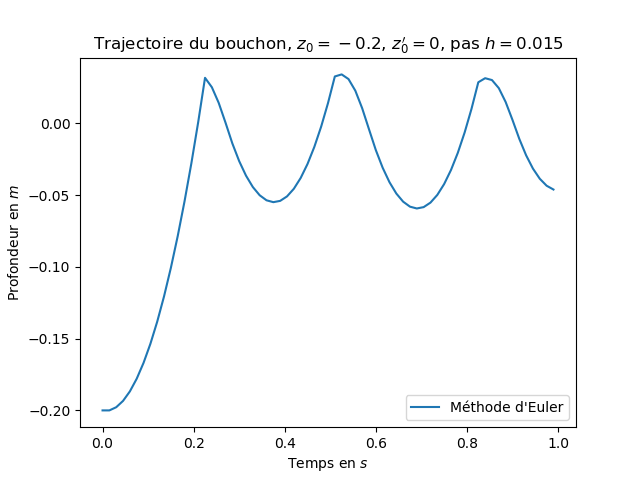
\includegraphics[width=.9\textwidth]{trajectoire.png}
        \caption{Trajectoire du bouchon au cours du temps.}
        \label{EQD-003:fig:trajectoire}
    \end{center}
\end{figure}

\question{} Commenter brièvement la cohérence physique d'une telle courbe. Pouvez-vous fournir une explication et une solution au problème observé, tout en restant dans le cadre de la méthode d'Euler ? 

% On donne sur la figure suivante (figures \ref{traj_bouchon} et \ref{portrait_bouchon}) le résultat (trajectoire et portrait de phase) de l'application de la méthode d'euler pour simuler le comportement de la chute libre d'un bouchon à partir de $5cm$ au dessus du niveau de l'eau.
% 
% 
% \question{} En supposant que les différentes fonctions demandées précédemment ont été correctement définies, donner la suite d'instruction permettant d'obtenir ces deux courbes.
% 
% \begin{figure}[!htb]
% \begin{minipage}{0.5\textwidth}
% \begin{center}
% 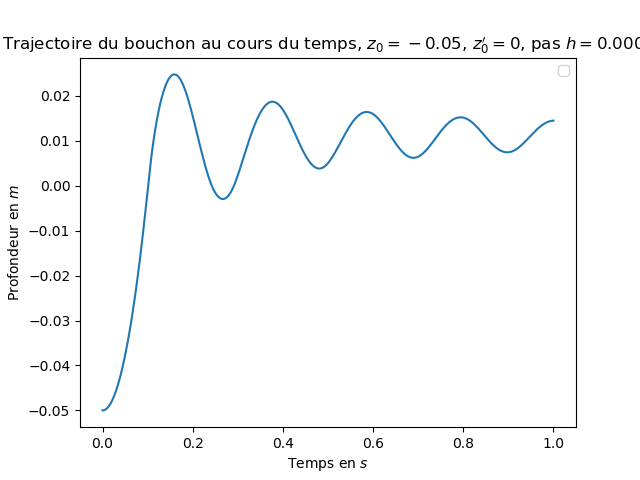
\includegraphics[width=0.9\textwidth]{z_t.png}
% \caption{Trajectoire du bouchon \label{traj_bouchon}}
% \end{center}
% \end{minipage}
% \begin{minipage}{0.5\textwidth}
% \begin{center}
% 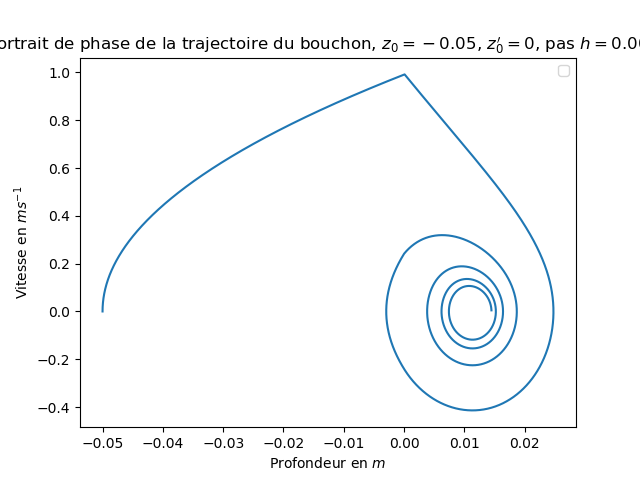
\includegraphics[width=0.9\textwidth]{portrait_de_phase.png}
% \caption{Portrait de phase du bouchon \label{portrait_bouchon}}
% \end{center}
% \end{minipage}

% \end{figure}


